\chapter{Gültigkeit und Einschränkungen}
\label{chap:gueltigkeit}

Es wird vom Erfolg der Nutzung des \gls{mmf} und \gls{arh} in diesem Fall mit \jf auf die generelle Nützlichkeit des Frameworks und Werkzeugs geschlossen.
Dabei gibt es neben der Qualität des \gls{mmf} und \gls{arh} viele andere Faktoren, die das Ergebnis im Einzelfall und auch in dieser Fallstudie beeinflussen können:

\begin{itemize}
	\item Die Auswahl der Migrationsmethode wird beeinflusst durch
	\begin{itemize}
		\item Qualität der \glspl{qa}
		\item Qualität der Filter
		\item Gleichgewicht zwischen \glspl{qa} und Filtern
	\end{itemize}
\end{itemize}

\begin{figure}
	\centering
	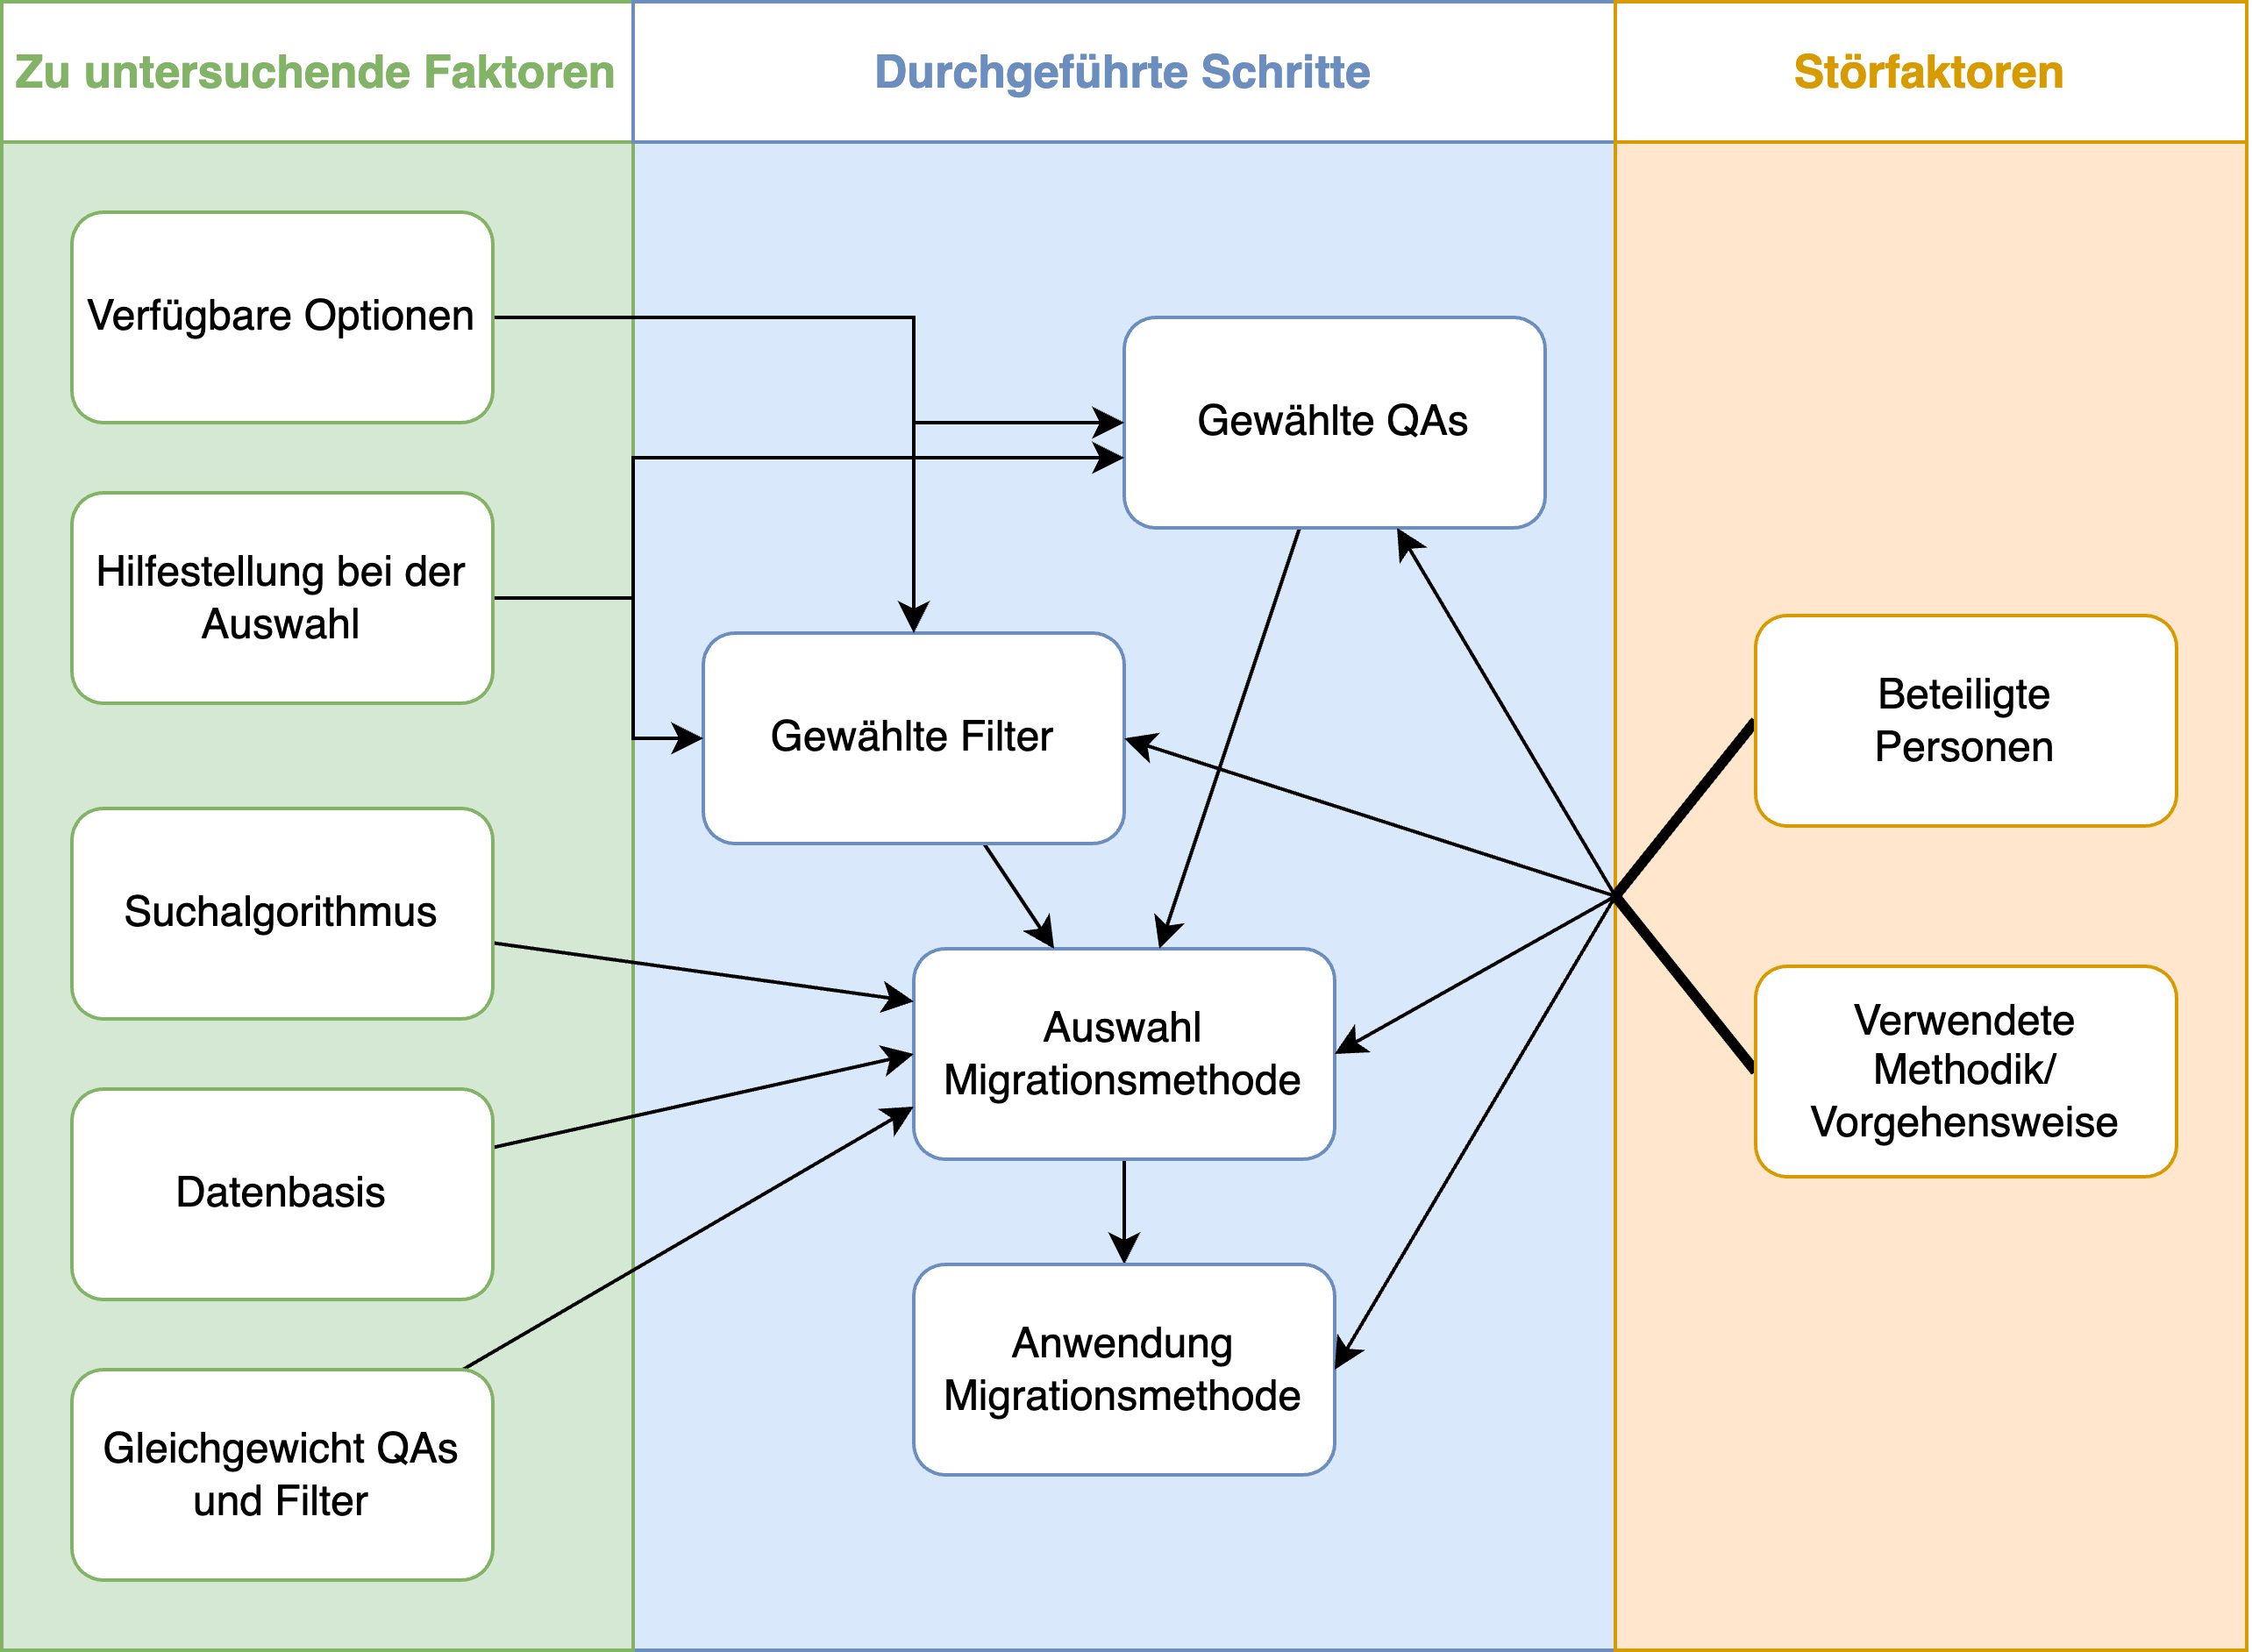
\includegraphics[width=1.0\textwidth]{limitations.drawio}
	\caption[Einflüsse auf das Ergebnis der Fallstudie]{
		Einflüsse der Qualität des \gls{mmf} und \gls{arh} sowie andere Einflüsse auf das Ergebnis der Fallstudie.
	}
	\label{fig:limitations}
\end{figure}

Phase 1:
Das Architekturreview ist für die Migration zu einem Microservices-System von Monolithen gedacht.
Insbesondere existiert dabei das Zielprodukt noch nicht in der Ziel Architektur. 
In unserem Fall dagegen war die Ausgangsarchitektur schon gleich der Zielarchitektur.
Dadurch war es bei dem Architekturreview schwierig, die technische Schwierigkeit eines Szenarios einzuschätzen, da einige der Szenarios so schon umgesetzt sind und damit argumentiert werden kann, dass es dann nicht technisch schwierig ist, da es schon vorhanden ist.

Nicht möglich gewesen, dass alle Stakeholder beim Architekturreview anwesend sind: Kein Kunde  

